% This TeX document is part of the manual of the GNU Astronomy
% Utilities (Gnuastro). A Makefile is also distributed which allows
% you to compile this TeX file in the desired manner.
%
% Original author:
%     Mohammad Akhlaghi <mohammad@akhlaghi.org>
% Contributing author(s):
% Copyright (C) 2022 Free Software Foundation, Inc.
%
% Gnuastro is free software: you can redistribute it and/or modify it
% under the terms of the GNU General Public License as published by
% the Free Software Foundation, either version 3 of the License, or
% (at your option) any later version.
%
% Gnuastro is distributed in the hope that it will be useful, but
% WITHOUT ANY WARRANTY; without even the implied warranty of
% MERCHANTABILITY or FITNESS FOR A PARTICULAR PURPOSE.  See the GNU
% General Public License for more details.
%
% You should have received a copy of the GNU General Public License
% along with Gnuastro. If not, see <http://www.gnu.org/licenses/>.





%% To generate the repetative parts of this file, we first wrote the output
%% of the '--listcolors' option of ConvertType into a table:
%%
%%     astconvertt --listcolors | asttable -ocolors.fits





%% Special color names to avoid confusing with standard color names. To
%% generate these, we used the 'colors.fits' above with the following
%% command:
%%
%%    asttable colors.fits -cColor-Name,FRAC-R,FRAC-G,Frac-B \
%%             | awk '{printf "\\definecolor{gnuastro%s}{rgb}{%.2f,%.2f,%.2f}\n", \
%%                            $1, $2, $3, $4}'
\definecolor{gnuastromediumvioletred}{rgb}{0.78,0.08,0.52}
\definecolor{gnuastrodeeppink}{rgb}{1.00,0.08,0.58}
\definecolor{gnuastropalevioletred}{rgb}{0.86,0.44,0.58}
\definecolor{gnuastrohotpink}{rgb}{1.00,0.41,0.71}
\definecolor{gnuastrolightpink}{rgb}{1.00,0.71,0.76}
\definecolor{gnuastropink}{rgb}{1.00,0.75,0.80}
\definecolor{gnuastrodarkred}{rgb}{0.55,0.00,0.00}
\definecolor{gnuastrored}{rgb}{1.00,0.00,0.00}
\definecolor{gnuastrofirebrick}{rgb}{0.70,0.13,0.13}
\definecolor{gnuastrocrimson}{rgb}{0.86,0.08,0.24}
\definecolor{gnuastroindianred}{rgb}{0.80,0.36,0.36}
\definecolor{gnuastrolightcoral}{rgb}{0.94,0.50,0.50}
\definecolor{gnuastrosalmon}{rgb}{0.98,0.50,0.45}
\definecolor{gnuastrodarksalmon}{rgb}{0.91,0.59,0.48}
\definecolor{gnuastrolightsalmon}{rgb}{1.00,0.63,0.48}
\definecolor{gnuastroorangered}{rgb}{1.00,0.27,0.00}
\definecolor{gnuastrotomato}{rgb}{1.00,0.39,0.28}
\definecolor{gnuastrodarkorange}{rgb}{1.00,0.55,0.00}
\definecolor{gnuastrocoral}{rgb}{1.00,0.50,0.31}
\definecolor{gnuastroorange}{rgb}{1.00,0.65,0.00}
\definecolor{gnuastrodarkkhaki}{rgb}{0.74,0.72,0.42}
\definecolor{gnuastrogold}{rgb}{1.00,0.84,0.00}
\definecolor{gnuastrokhaki}{rgb}{0.94,0.90,0.55}
\definecolor{gnuastropeachpuff}{rgb}{1.00,0.85,0.73}
\definecolor{gnuastroyellow}{rgb}{1.00,1.00,0.00}
\definecolor{gnuastropalegoldenrod}{rgb}{0.93,0.91,0.67}
\definecolor{gnuastromoccasin}{rgb}{1.00,0.89,0.71}
\definecolor{gnuastropapayawhip}{rgb}{1.00,0.94,0.84}
\definecolor{gnuastrolightgoldenrodyellow}{rgb}{0.98,0.98,0.82}
\definecolor{gnuastrolemonchiffon}{rgb}{1.00,0.98,0.80}
\definecolor{gnuastrolightyellow}{rgb}{1.00,1.00,0.88}
\definecolor{gnuastromaroon}{rgb}{0.50,0.00,0.00}
\definecolor{gnuastrobrown}{rgb}{0.65,0.16,0.16}
\definecolor{gnuastrosaddlebrown}{rgb}{0.55,0.27,0.07}
\definecolor{gnuastrosienna}{rgb}{0.63,0.32,0.18}
\definecolor{gnuastrochocolate}{rgb}{0.82,0.41,0.12}
\definecolor{gnuastrodarkgoldenrod}{rgb}{0.72,0.53,0.04}
\definecolor{gnuastroperu}{rgb}{0.80,0.52,0.25}
\definecolor{gnuastrorosybrown}{rgb}{0.74,0.56,0.56}
\definecolor{gnuastrogoldenrod}{rgb}{0.85,0.65,0.13}
\definecolor{gnuastrosandybrown}{rgb}{0.96,0.64,0.38}
\definecolor{gnuastrotan}{rgb}{0.82,0.71,0.55}
\definecolor{gnuastroburlywood}{rgb}{0.87,0.72,0.53}
\definecolor{gnuastrowheat}{rgb}{0.96,0.87,0.70}
\definecolor{gnuastronavajowhite}{rgb}{1.00,0.87,0.68}
\definecolor{gnuastrobisque}{rgb}{1.00,0.89,0.77}
\definecolor{gnuastroblanchedalmond}{rgb}{1.00,0.92,0.80}
\definecolor{gnuastrocornsilk}{rgb}{1.00,0.97,0.86}
\definecolor{gnuastrodarkgreen}{rgb}{0.00,0.39,0.00}
\definecolor{gnuastrogreen}{rgb}{0.00,0.50,0.00}
\definecolor{gnuastrodarkolivegreen}{rgb}{0.33,0.42,0.18}
\definecolor{gnuastroforestgreen}{rgb}{0.13,0.55,0.13}
\definecolor{gnuastroseagreen}{rgb}{0.18,0.55,0.34}
\definecolor{gnuastroolive}{rgb}{0.50,0.50,0.00}
\definecolor{gnuastroolivedrab}{rgb}{0.42,0.56,0.14}
\definecolor{gnuastromediumseagreen}{rgb}{0.24,0.70,0.44}
\definecolor{gnuastrolimegreen}{rgb}{0.20,0.80,0.20}
\definecolor{gnuastrolime}{rgb}{0.00,1.00,0.00}
\definecolor{gnuastrospringgreen}{rgb}{0.00,1.00,0.50}
\definecolor{gnuastromediumspringgreen}{rgb}{0.00,0.98,0.60}
\definecolor{gnuastrodarkseagreen}{rgb}{0.56,0.74,0.56}
\definecolor{gnuastromediumaquamarine}{rgb}{0.40,0.80,0.67}
\definecolor{gnuastroyellowgreen}{rgb}{0.60,0.80,0.20}
\definecolor{gnuastrolawngreen}{rgb}{0.49,0.99,0.00}
\definecolor{gnuastrochartreuse}{rgb}{0.50,1.00,0.00}
\definecolor{gnuastrolightgreen}{rgb}{0.56,0.93,0.56}
\definecolor{gnuastrogreenyellow}{rgb}{0.68,1.00,0.18}
\definecolor{gnuastropalegreen}{rgb}{0.60,0.98,0.60}
\definecolor{gnuastroteal}{rgb}{0.00,0.50,0.50}
\definecolor{gnuastrodarkcyan}{rgb}{0.00,0.55,0.55}
\definecolor{gnuastrolightseagreen}{rgb}{0.13,0.70,0.67}
\definecolor{gnuastrocadetblue}{rgb}{0.37,0.62,0.63}
\definecolor{gnuastrodarkturquoise}{rgb}{0.00,0.81,0.82}
\definecolor{gnuastromediumturquoise}{rgb}{0.28,0.82,0.80}
\definecolor{gnuastroturquoise}{rgb}{0.25,0.88,0.82}
\definecolor{gnuastroaqua}{rgb}{0.00,1.00,1.00}
\definecolor{gnuastrocyan}{rgb}{0.00,1.00,1.00}
\definecolor{gnuastroaquamarine}{rgb}{0.50,1.00,0.83}
\definecolor{gnuastropaleturquoise}{rgb}{0.69,0.93,0.93}
\definecolor{gnuastrolightcyan}{rgb}{0.88,1.00,1.00}
\definecolor{gnuastromidnightblue}{rgb}{0.10,0.10,0.44}
\definecolor{gnuastronavy}{rgb}{0.00,0.00,0.50}
\definecolor{gnuastrodarkblue}{rgb}{0.00,0.00,0.55}
\definecolor{gnuastromediumblue}{rgb}{0.00,0.00,0.80}
\definecolor{gnuastroblue}{rgb}{0.00,0.00,1.00}
\definecolor{gnuastroroyalblue}{rgb}{0.25,0.41,0.88}
\definecolor{gnuastrosteelblue}{rgb}{0.27,0.51,0.71}
\definecolor{gnuastrododgerblue}{rgb}{0.12,0.56,1.00}
\definecolor{gnuastrodeepskyblue}{rgb}{0.00,0.75,1.00}
\definecolor{gnuastrocornflowerblue}{rgb}{0.39,0.58,0.93}
\definecolor{gnuastroskyblue}{rgb}{0.53,0.81,0.92}
\definecolor{gnuastrolightskyblue}{rgb}{0.53,0.81,0.98}
\definecolor{gnuastrolightsteelblue}{rgb}{0.69,0.77,0.87}
\definecolor{gnuastrolightblue}{rgb}{0.68,0.85,0.90}
\definecolor{gnuastropowderblue}{rgb}{0.69,0.88,0.90}
\definecolor{gnuastroindigo}{rgb}{0.29,0.00,0.51}
\definecolor{gnuastropurple}{rgb}{0.50,0.00,0.50}
\definecolor{gnuastrodarkmagenta}{rgb}{0.55,0.00,0.55}
\definecolor{gnuastrodarkviolet}{rgb}{0.58,0.00,0.83}
\definecolor{gnuastrodarkslateblue}{rgb}{0.28,0.24,0.55}
\definecolor{gnuastroblueviolet}{rgb}{0.54,0.17,0.89}
\definecolor{gnuastrodarkorchid}{rgb}{0.60,0.20,0.80}
\definecolor{gnuastrofuchsia}{rgb}{1.00,0.00,1.00}
\definecolor{gnuastromagenta}{rgb}{1.00,0.00,1.00}
\definecolor{gnuastroslateblue}{rgb}{0.42,0.35,0.80}
\definecolor{gnuastromediumslateblue}{rgb}{0.48,0.41,0.93}
\definecolor{gnuastromediumorchid}{rgb}{0.73,0.33,0.83}
\definecolor{gnuastromediumpurple}{rgb}{0.58,0.44,0.86}
\definecolor{gnuastroorchid}{rgb}{0.85,0.44,0.84}
\definecolor{gnuastroviolet}{rgb}{0.93,0.51,0.93}
\definecolor{gnuastroplum}{rgb}{0.87,0.63,0.87}
\definecolor{gnuastrothistle}{rgb}{0.85,0.75,0.85}
\definecolor{gnuastrolavender}{rgb}{0.90,0.90,0.98}
\definecolor{gnuastromistyrose}{rgb}{1.00,0.89,0.88}
\definecolor{gnuastroantiquewhite}{rgb}{0.98,0.92,0.84}
\definecolor{gnuastrolinen}{rgb}{0.98,0.94,0.90}
\definecolor{gnuastrobeige}{rgb}{0.96,0.96,0.86}
\definecolor{gnuastrowhitesmoke}{rgb}{0.96,0.96,0.96}
\definecolor{gnuastrolavenderblush}{rgb}{1.00,0.94,0.96}
\definecolor{gnuastrooldlace}{rgb}{0.99,0.96,0.90}
\definecolor{gnuastroaliceblue}{rgb}{0.94,0.97,1.00}
\definecolor{gnuastroseashell}{rgb}{1.00,0.96,0.93}
\definecolor{gnuastroghostwhite}{rgb}{0.97,0.97,1.00}
\definecolor{gnuastrohoneydew}{rgb}{0.94,1.00,0.94}
\definecolor{gnuastrofloralwhite}{rgb}{1.00,0.98,0.94}
\definecolor{gnuastroazure}{rgb}{0.94,1.00,1.00}
\definecolor{gnuastromintcream}{rgb}{0.96,1.00,0.98}
\definecolor{gnuastrosnow}{rgb}{1.00,0.98,0.98}
\definecolor{gnuastroivory}{rgb}{1.00,1.00,0.94}
\definecolor{gnuastrowhite}{rgb}{1.00,1.00,1.00}
\definecolor{gnuastroblack}{rgb}{0.00,0.00,0.00}
\definecolor{gnuastrodarkslategray}{rgb}{0.18,0.31,0.31}
\definecolor{gnuastrodimgray}{rgb}{0.41,0.41,0.41}
\definecolor{gnuastroslategray}{rgb}{0.44,0.50,0.56}
\definecolor{gnuastrogray}{rgb}{0.50,0.50,0.50}
\definecolor{gnuastrolightslategray}{rgb}{0.47,0.53,0.60}
\definecolor{gnuastrodarkgray}{rgb}{0.66,0.66,0.66}
\definecolor{gnuastrosilver}{rgb}{0.75,0.75,0.75}
\definecolor{gnuastrolightgray}{rgb}{0.83,0.83,0.83}
\definecolor{gnuastrogainsboro}{rgb}{0.86,0.86,0.86}



%% Using the 'colors.fits' file above, the repetative parts below were
%% constructed with this command. Colors with long names will be treated
%% specially: their code will be printed in the next line.
%%
%% asttable colors.fits -cColor-ID,Color-Name \
%%     | awk -vspacing=0.008 -vboxw=0.02 -vnrows=20 -vcolwidth=0.18 \
%%           '{ \
%%              if( $2=="lightgoldenrodyellow" \
%%                  || $2=="mediumspringgreen" ) { \
%% 	       special=1;
%%              } \
%% 	     else special=0; \
%%              printf("\\draw [fill=gnuastro%s] (%f\\linewidth,%f\\linewidth) rectangle (%f\\linewidth,%f\\linewidth);\n", \
%%                     $2, x, y, x+boxw, y+boxw); \
%%              printf("\\draw [anchor=south west, inner sep=1, outer sep=0] (%f\\linewidth,%f\\linewidth) node {\\texttt{%s%s}};\n", \
%%                         x+boxw, y, $2, special==0?" ("$1")":""); \
%%              if(special==1) \
%%                printf("\\draw [anchor=south west, inner sep=0, outer sep=0] (%f\\linewidth,%f\\linewidth) node {\\texttt{(%d)}};\n", \
%%                         x+boxw, y-boxw/2, NR); \
%%              y-=boxw+spacing; \
%%              if(NR%nrows==0) {x+=colwidth; y=0} }' > colors.tex
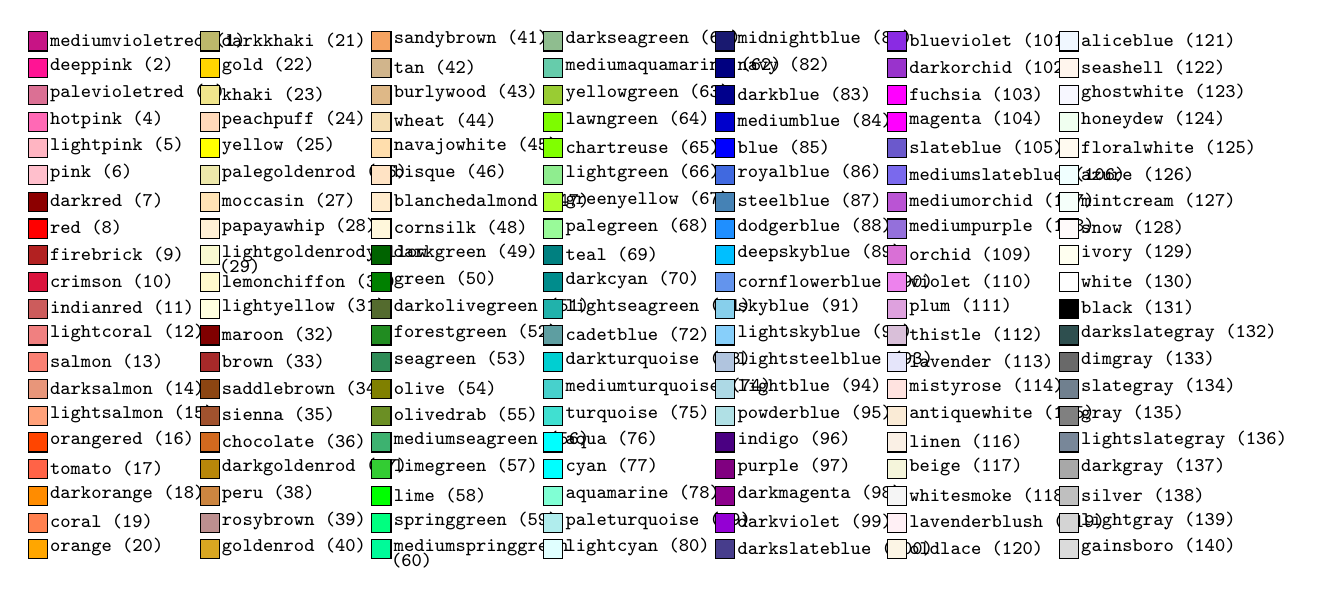
\begin{tikzpicture}
\scriptsize
\draw [fill=gnuastromediumvioletred] (0.000000\linewidth,0.000000\linewidth) rectangle (0.020000\linewidth,0.020000\linewidth);
\draw [anchor=south west, inner sep=1, outer sep=0] (0.020000\linewidth,0.000000\linewidth) node {\texttt{mediumvioletred (1)}};
\draw [fill=gnuastrodeeppink] (0.000000\linewidth,-0.028000\linewidth) rectangle (0.020000\linewidth,-0.008000\linewidth);
\draw [anchor=south west, inner sep=1, outer sep=0] (0.020000\linewidth,-0.028000\linewidth) node {\texttt{deeppink (2)}};
\draw [fill=gnuastropalevioletred] (0.000000\linewidth,-0.056000\linewidth) rectangle (0.020000\linewidth,-0.036000\linewidth);
\draw [anchor=south west, inner sep=1, outer sep=0] (0.020000\linewidth,-0.056000\linewidth) node {\texttt{palevioletred (3)}};
\draw [fill=gnuastrohotpink] (0.000000\linewidth,-0.084000\linewidth) rectangle (0.020000\linewidth,-0.064000\linewidth);
\draw [anchor=south west, inner sep=1, outer sep=0] (0.020000\linewidth,-0.084000\linewidth) node {\texttt{hotpink (4)}};
\draw [fill=gnuastrolightpink] (0.000000\linewidth,-0.112000\linewidth) rectangle (0.020000\linewidth,-0.092000\linewidth);
\draw [anchor=south west, inner sep=1, outer sep=0] (0.020000\linewidth,-0.112000\linewidth) node {\texttt{lightpink (5)}};
\draw [fill=gnuastropink] (0.000000\linewidth,-0.140000\linewidth) rectangle (0.020000\linewidth,-0.120000\linewidth);
\draw [anchor=south west, inner sep=1, outer sep=0] (0.020000\linewidth,-0.140000\linewidth) node {\texttt{pink (6)}};
\draw [fill=gnuastrodarkred] (0.000000\linewidth,-0.168000\linewidth) rectangle (0.020000\linewidth,-0.148000\linewidth);
\draw [anchor=south west, inner sep=1, outer sep=0] (0.020000\linewidth,-0.168000\linewidth) node {\texttt{darkred (7)}};
\draw [fill=gnuastrored] (0.000000\linewidth,-0.196000\linewidth) rectangle (0.020000\linewidth,-0.176000\linewidth);
\draw [anchor=south west, inner sep=1, outer sep=0] (0.020000\linewidth,-0.196000\linewidth) node {\texttt{red (8)}};
\draw [fill=gnuastrofirebrick] (0.000000\linewidth,-0.224000\linewidth) rectangle (0.020000\linewidth,-0.204000\linewidth);
\draw [anchor=south west, inner sep=1, outer sep=0] (0.020000\linewidth,-0.224000\linewidth) node {\texttt{firebrick (9)}};
\draw [fill=gnuastrocrimson] (0.000000\linewidth,-0.252000\linewidth) rectangle (0.020000\linewidth,-0.232000\linewidth);
\draw [anchor=south west, inner sep=1, outer sep=0] (0.020000\linewidth,-0.252000\linewidth) node {\texttt{crimson (10)}};
\draw [fill=gnuastroindianred] (0.000000\linewidth,-0.280000\linewidth) rectangle (0.020000\linewidth,-0.260000\linewidth);
\draw [anchor=south west, inner sep=1, outer sep=0] (0.020000\linewidth,-0.280000\linewidth) node {\texttt{indianred (11)}};
\draw [fill=gnuastrolightcoral] (0.000000\linewidth,-0.308000\linewidth) rectangle (0.020000\linewidth,-0.288000\linewidth);
\draw [anchor=south west, inner sep=1, outer sep=0] (0.020000\linewidth,-0.308000\linewidth) node {\texttt{lightcoral (12)}};
\draw [fill=gnuastrosalmon] (0.000000\linewidth,-0.336000\linewidth) rectangle (0.020000\linewidth,-0.316000\linewidth);
\draw [anchor=south west, inner sep=1, outer sep=0] (0.020000\linewidth,-0.336000\linewidth) node {\texttt{salmon (13)}};
\draw [fill=gnuastrodarksalmon] (0.000000\linewidth,-0.364000\linewidth) rectangle (0.020000\linewidth,-0.344000\linewidth);
\draw [anchor=south west, inner sep=1, outer sep=0] (0.020000\linewidth,-0.364000\linewidth) node {\texttt{darksalmon (14)}};
\draw [fill=gnuastrolightsalmon] (0.000000\linewidth,-0.392000\linewidth) rectangle (0.020000\linewidth,-0.372000\linewidth);
\draw [anchor=south west, inner sep=1, outer sep=0] (0.020000\linewidth,-0.392000\linewidth) node {\texttt{lightsalmon (15)}};
\draw [fill=gnuastroorangered] (0.000000\linewidth,-0.420000\linewidth) rectangle (0.020000\linewidth,-0.400000\linewidth);
\draw [anchor=south west, inner sep=1, outer sep=0] (0.020000\linewidth,-0.420000\linewidth) node {\texttt{orangered (16)}};
\draw [fill=gnuastrotomato] (0.000000\linewidth,-0.448000\linewidth) rectangle (0.020000\linewidth,-0.428000\linewidth);
\draw [anchor=south west, inner sep=1, outer sep=0] (0.020000\linewidth,-0.448000\linewidth) node {\texttt{tomato (17)}};
\draw [fill=gnuastrodarkorange] (0.000000\linewidth,-0.476000\linewidth) rectangle (0.020000\linewidth,-0.456000\linewidth);
\draw [anchor=south west, inner sep=1, outer sep=0] (0.020000\linewidth,-0.476000\linewidth) node {\texttt{darkorange (18)}};
\draw [fill=gnuastrocoral] (0.000000\linewidth,-0.504000\linewidth) rectangle (0.020000\linewidth,-0.484000\linewidth);
\draw [anchor=south west, inner sep=1, outer sep=0] (0.020000\linewidth,-0.504000\linewidth) node {\texttt{coral (19)}};
\draw [fill=gnuastroorange] (0.000000\linewidth,-0.532000\linewidth) rectangle (0.020000\linewidth,-0.512000\linewidth);
\draw [anchor=south west, inner sep=1, outer sep=0] (0.020000\linewidth,-0.532000\linewidth) node {\texttt{orange (20)}};
\draw [fill=gnuastrodarkkhaki] (0.180000\linewidth,0.000000\linewidth) rectangle (0.200000\linewidth,0.020000\linewidth);
\draw [anchor=south west, inner sep=1, outer sep=0] (0.200000\linewidth,0.000000\linewidth) node {\texttt{darkkhaki (21)}};
\draw [fill=gnuastrogold] (0.180000\linewidth,-0.028000\linewidth) rectangle (0.200000\linewidth,-0.008000\linewidth);
\draw [anchor=south west, inner sep=1, outer sep=0] (0.200000\linewidth,-0.028000\linewidth) node {\texttt{gold (22)}};
\draw [fill=gnuastrokhaki] (0.180000\linewidth,-0.056000\linewidth) rectangle (0.200000\linewidth,-0.036000\linewidth);
\draw [anchor=south west, inner sep=1, outer sep=0] (0.200000\linewidth,-0.056000\linewidth) node {\texttt{khaki (23)}};
\draw [fill=gnuastropeachpuff] (0.180000\linewidth,-0.084000\linewidth) rectangle (0.200000\linewidth,-0.064000\linewidth);
\draw [anchor=south west, inner sep=1, outer sep=0] (0.200000\linewidth,-0.084000\linewidth) node {\texttt{peachpuff (24)}};
\draw [fill=gnuastroyellow] (0.180000\linewidth,-0.112000\linewidth) rectangle (0.200000\linewidth,-0.092000\linewidth);
\draw [anchor=south west, inner sep=1, outer sep=0] (0.200000\linewidth,-0.112000\linewidth) node {\texttt{yellow (25)}};
\draw [fill=gnuastropalegoldenrod] (0.180000\linewidth,-0.140000\linewidth) rectangle (0.200000\linewidth,-0.120000\linewidth);
\draw [anchor=south west, inner sep=1, outer sep=0] (0.200000\linewidth,-0.140000\linewidth) node {\texttt{palegoldenrod (26)}};
\draw [fill=gnuastromoccasin] (0.180000\linewidth,-0.168000\linewidth) rectangle (0.200000\linewidth,-0.148000\linewidth);
\draw [anchor=south west, inner sep=1, outer sep=0] (0.200000\linewidth,-0.168000\linewidth) node {\texttt{moccasin (27)}};
\draw [fill=gnuastropapayawhip] (0.180000\linewidth,-0.196000\linewidth) rectangle (0.200000\linewidth,-0.176000\linewidth);
\draw [anchor=south west, inner sep=1, outer sep=0] (0.200000\linewidth,-0.196000\linewidth) node {\texttt{papayawhip (28)}};
\draw [fill=gnuastrolightgoldenrodyellow] (0.180000\linewidth,-0.224000\linewidth) rectangle (0.200000\linewidth,-0.204000\linewidth);
\draw [anchor=south west, inner sep=1, outer sep=0] (0.200000\linewidth,-0.224000\linewidth) node {\texttt{lightgoldenrodyellow}};
\draw [anchor=south west, inner sep=0, outer sep=0] (0.200000\linewidth,-0.234000\linewidth) node {\texttt{(29)}};
\draw [fill=gnuastrolemonchiffon] (0.180000\linewidth,-0.252000\linewidth) rectangle (0.200000\linewidth,-0.232000\linewidth);
\draw [anchor=south west, inner sep=1, outer sep=0] (0.200000\linewidth,-0.252000\linewidth) node {\texttt{lemonchiffon (30)}};
\draw [fill=gnuastrolightyellow] (0.180000\linewidth,-0.280000\linewidth) rectangle (0.200000\linewidth,-0.260000\linewidth);
\draw [anchor=south west, inner sep=1, outer sep=0] (0.200000\linewidth,-0.280000\linewidth) node {\texttt{lightyellow (31)}};
\draw [fill=gnuastromaroon] (0.180000\linewidth,-0.308000\linewidth) rectangle (0.200000\linewidth,-0.288000\linewidth);
\draw [anchor=south west, inner sep=1, outer sep=0] (0.200000\linewidth,-0.308000\linewidth) node {\texttt{maroon (32)}};
\draw [fill=gnuastrobrown] (0.180000\linewidth,-0.336000\linewidth) rectangle (0.200000\linewidth,-0.316000\linewidth);
\draw [anchor=south west, inner sep=1, outer sep=0] (0.200000\linewidth,-0.336000\linewidth) node {\texttt{brown (33)}};
\draw [fill=gnuastrosaddlebrown] (0.180000\linewidth,-0.364000\linewidth) rectangle (0.200000\linewidth,-0.344000\linewidth);
\draw [anchor=south west, inner sep=1, outer sep=0] (0.200000\linewidth,-0.364000\linewidth) node {\texttt{saddlebrown (34)}};
\draw [fill=gnuastrosienna] (0.180000\linewidth,-0.392000\linewidth) rectangle (0.200000\linewidth,-0.372000\linewidth);
\draw [anchor=south west, inner sep=1, outer sep=0] (0.200000\linewidth,-0.392000\linewidth) node {\texttt{sienna (35)}};
\draw [fill=gnuastrochocolate] (0.180000\linewidth,-0.420000\linewidth) rectangle (0.200000\linewidth,-0.400000\linewidth);
\draw [anchor=south west, inner sep=1, outer sep=0] (0.200000\linewidth,-0.420000\linewidth) node {\texttt{chocolate (36)}};
\draw [fill=gnuastrodarkgoldenrod] (0.180000\linewidth,-0.448000\linewidth) rectangle (0.200000\linewidth,-0.428000\linewidth);
\draw [anchor=south west, inner sep=1, outer sep=0] (0.200000\linewidth,-0.448000\linewidth) node {\texttt{darkgoldenrod (37)}};
\draw [fill=gnuastroperu] (0.180000\linewidth,-0.476000\linewidth) rectangle (0.200000\linewidth,-0.456000\linewidth);
\draw [anchor=south west, inner sep=1, outer sep=0] (0.200000\linewidth,-0.476000\linewidth) node {\texttt{peru (38)}};
\draw [fill=gnuastrorosybrown] (0.180000\linewidth,-0.504000\linewidth) rectangle (0.200000\linewidth,-0.484000\linewidth);
\draw [anchor=south west, inner sep=1, outer sep=0] (0.200000\linewidth,-0.504000\linewidth) node {\texttt{rosybrown (39)}};
\draw [fill=gnuastrogoldenrod] (0.180000\linewidth,-0.532000\linewidth) rectangle (0.200000\linewidth,-0.512000\linewidth);
\draw [anchor=south west, inner sep=1, outer sep=0] (0.200000\linewidth,-0.532000\linewidth) node {\texttt{goldenrod (40)}};
\draw [fill=gnuastrosandybrown] (0.360000\linewidth,0.000000\linewidth) rectangle (0.380000\linewidth,0.020000\linewidth);
\draw [anchor=south west, inner sep=1, outer sep=0] (0.380000\linewidth,0.000000\linewidth) node {\texttt{sandybrown (41)}};
\draw [fill=gnuastrotan] (0.360000\linewidth,-0.028000\linewidth) rectangle (0.380000\linewidth,-0.008000\linewidth);
\draw [anchor=south west, inner sep=1, outer sep=0] (0.380000\linewidth,-0.028000\linewidth) node {\texttt{tan (42)}};
\draw [fill=gnuastroburlywood] (0.360000\linewidth,-0.056000\linewidth) rectangle (0.380000\linewidth,-0.036000\linewidth);
\draw [anchor=south west, inner sep=1, outer sep=0] (0.380000\linewidth,-0.056000\linewidth) node {\texttt{burlywood (43)}};
\draw [fill=gnuastrowheat] (0.360000\linewidth,-0.084000\linewidth) rectangle (0.380000\linewidth,-0.064000\linewidth);
\draw [anchor=south west, inner sep=1, outer sep=0] (0.380000\linewidth,-0.084000\linewidth) node {\texttt{wheat (44)}};
\draw [fill=gnuastronavajowhite] (0.360000\linewidth,-0.112000\linewidth) rectangle (0.380000\linewidth,-0.092000\linewidth);
\draw [anchor=south west, inner sep=1, outer sep=0] (0.380000\linewidth,-0.112000\linewidth) node {\texttt{navajowhite (45)}};
\draw [fill=gnuastrobisque] (0.360000\linewidth,-0.140000\linewidth) rectangle (0.380000\linewidth,-0.120000\linewidth);
\draw [anchor=south west, inner sep=1, outer sep=0] (0.380000\linewidth,-0.140000\linewidth) node {\texttt{bisque (46)}};
\draw [fill=gnuastroblanchedalmond] (0.360000\linewidth,-0.168000\linewidth) rectangle (0.380000\linewidth,-0.148000\linewidth);
\draw [anchor=south west, inner sep=1, outer sep=0] (0.380000\linewidth,-0.168000\linewidth) node {\texttt{blanchedalmond (47)}};
\draw [fill=gnuastrocornsilk] (0.360000\linewidth,-0.196000\linewidth) rectangle (0.380000\linewidth,-0.176000\linewidth);
\draw [anchor=south west, inner sep=1, outer sep=0] (0.380000\linewidth,-0.196000\linewidth) node {\texttt{cornsilk (48)}};
\draw [fill=gnuastrodarkgreen] (0.360000\linewidth,-0.224000\linewidth) rectangle (0.380000\linewidth,-0.204000\linewidth);
\draw [anchor=south west, inner sep=1, outer sep=0] (0.380000\linewidth,-0.224000\linewidth) node {\texttt{darkgreen (49)}};
\draw [fill=gnuastrogreen] (0.360000\linewidth,-0.252000\linewidth) rectangle (0.380000\linewidth,-0.232000\linewidth);
\draw [anchor=south west, inner sep=1, outer sep=0] (0.380000\linewidth,-0.252000\linewidth) node {\texttt{green (50)}};
\draw [fill=gnuastrodarkolivegreen] (0.360000\linewidth,-0.280000\linewidth) rectangle (0.380000\linewidth,-0.260000\linewidth);
\draw [anchor=south west, inner sep=1, outer sep=0] (0.380000\linewidth,-0.280000\linewidth) node {\texttt{darkolivegreen (51)}};
\draw [fill=gnuastroforestgreen] (0.360000\linewidth,-0.308000\linewidth) rectangle (0.380000\linewidth,-0.288000\linewidth);
\draw [anchor=south west, inner sep=1, outer sep=0] (0.380000\linewidth,-0.308000\linewidth) node {\texttt{forestgreen (52)}};
\draw [fill=gnuastroseagreen] (0.360000\linewidth,-0.336000\linewidth) rectangle (0.380000\linewidth,-0.316000\linewidth);
\draw [anchor=south west, inner sep=1, outer sep=0] (0.380000\linewidth,-0.336000\linewidth) node {\texttt{seagreen (53)}};
\draw [fill=gnuastroolive] (0.360000\linewidth,-0.364000\linewidth) rectangle (0.380000\linewidth,-0.344000\linewidth);
\draw [anchor=south west, inner sep=1, outer sep=0] (0.380000\linewidth,-0.364000\linewidth) node {\texttt{olive (54)}};
\draw [fill=gnuastroolivedrab] (0.360000\linewidth,-0.392000\linewidth) rectangle (0.380000\linewidth,-0.372000\linewidth);
\draw [anchor=south west, inner sep=1, outer sep=0] (0.380000\linewidth,-0.392000\linewidth) node {\texttt{olivedrab (55)}};
\draw [fill=gnuastromediumseagreen] (0.360000\linewidth,-0.420000\linewidth) rectangle (0.380000\linewidth,-0.400000\linewidth);
\draw [anchor=south west, inner sep=1, outer sep=0] (0.380000\linewidth,-0.420000\linewidth) node {\texttt{mediumseagreen (56)}};
\draw [fill=gnuastrolimegreen] (0.360000\linewidth,-0.448000\linewidth) rectangle (0.380000\linewidth,-0.428000\linewidth);
\draw [anchor=south west, inner sep=1, outer sep=0] (0.380000\linewidth,-0.448000\linewidth) node {\texttt{limegreen (57)}};
\draw [fill=gnuastrolime] (0.360000\linewidth,-0.476000\linewidth) rectangle (0.380000\linewidth,-0.456000\linewidth);
\draw [anchor=south west, inner sep=1, outer sep=0] (0.380000\linewidth,-0.476000\linewidth) node {\texttt{lime (58)}};
\draw [fill=gnuastrospringgreen] (0.360000\linewidth,-0.504000\linewidth) rectangle (0.380000\linewidth,-0.484000\linewidth);
\draw [anchor=south west, inner sep=1, outer sep=0] (0.380000\linewidth,-0.504000\linewidth) node {\texttt{springgreen (59)}};
\draw [fill=gnuastromediumspringgreen] (0.360000\linewidth,-0.532000\linewidth) rectangle (0.380000\linewidth,-0.512000\linewidth);
\draw [anchor=south west, inner sep=1, outer sep=0] (0.380000\linewidth,-0.532000\linewidth) node {\texttt{mediumspringgreen}};
\draw [anchor=south west, inner sep=0, outer sep=0] (0.380000\linewidth,-0.542000\linewidth) node {\texttt{(60)}};
\draw [fill=gnuastrodarkseagreen] (0.540000\linewidth,0.000000\linewidth) rectangle (0.560000\linewidth,0.020000\linewidth);
\draw [anchor=south west, inner sep=1, outer sep=0] (0.560000\linewidth,0.000000\linewidth) node {\texttt{darkseagreen (61)}};
\draw [fill=gnuastromediumaquamarine] (0.540000\linewidth,-0.028000\linewidth) rectangle (0.560000\linewidth,-0.008000\linewidth);
\draw [anchor=south west, inner sep=1, outer sep=0] (0.560000\linewidth,-0.028000\linewidth) node {\texttt{mediumaquamarine (62)}};
\draw [fill=gnuastroyellowgreen] (0.540000\linewidth,-0.056000\linewidth) rectangle (0.560000\linewidth,-0.036000\linewidth);
\draw [anchor=south west, inner sep=1, outer sep=0] (0.560000\linewidth,-0.056000\linewidth) node {\texttt{yellowgreen (63)}};
\draw [fill=gnuastrolawngreen] (0.540000\linewidth,-0.084000\linewidth) rectangle (0.560000\linewidth,-0.064000\linewidth);
\draw [anchor=south west, inner sep=1, outer sep=0] (0.560000\linewidth,-0.084000\linewidth) node {\texttt{lawngreen (64)}};
\draw [fill=gnuastrochartreuse] (0.540000\linewidth,-0.112000\linewidth) rectangle (0.560000\linewidth,-0.092000\linewidth);
\draw [anchor=south west, inner sep=1, outer sep=0] (0.560000\linewidth,-0.112000\linewidth) node {\texttt{chartreuse (65)}};
\draw [fill=gnuastrolightgreen] (0.540000\linewidth,-0.140000\linewidth) rectangle (0.560000\linewidth,-0.120000\linewidth);
\draw [anchor=south west, inner sep=1, outer sep=0] (0.560000\linewidth,-0.140000\linewidth) node {\texttt{lightgreen (66)}};
\draw [fill=gnuastrogreenyellow] (0.540000\linewidth,-0.168000\linewidth) rectangle (0.560000\linewidth,-0.148000\linewidth);
\draw [anchor=south west, inner sep=1, outer sep=0] (0.560000\linewidth,-0.168000\linewidth) node {\texttt{greenyellow (67)}};
\draw [fill=gnuastropalegreen] (0.540000\linewidth,-0.196000\linewidth) rectangle (0.560000\linewidth,-0.176000\linewidth);
\draw [anchor=south west, inner sep=1, outer sep=0] (0.560000\linewidth,-0.196000\linewidth) node {\texttt{palegreen (68)}};
\draw [fill=gnuastroteal] (0.540000\linewidth,-0.224000\linewidth) rectangle (0.560000\linewidth,-0.204000\linewidth);
\draw [anchor=south west, inner sep=1, outer sep=0] (0.560000\linewidth,-0.224000\linewidth) node {\texttt{teal (69)}};
\draw [fill=gnuastrodarkcyan] (0.540000\linewidth,-0.252000\linewidth) rectangle (0.560000\linewidth,-0.232000\linewidth);
\draw [anchor=south west, inner sep=1, outer sep=0] (0.560000\linewidth,-0.252000\linewidth) node {\texttt{darkcyan (70)}};
\draw [fill=gnuastrolightseagreen] (0.540000\linewidth,-0.280000\linewidth) rectangle (0.560000\linewidth,-0.260000\linewidth);
\draw [anchor=south west, inner sep=1, outer sep=0] (0.560000\linewidth,-0.280000\linewidth) node {\texttt{lightseagreen (71)}};
\draw [fill=gnuastrocadetblue] (0.540000\linewidth,-0.308000\linewidth) rectangle (0.560000\linewidth,-0.288000\linewidth);
\draw [anchor=south west, inner sep=1, outer sep=0] (0.560000\linewidth,-0.308000\linewidth) node {\texttt{cadetblue (72)}};
\draw [fill=gnuastrodarkturquoise] (0.540000\linewidth,-0.336000\linewidth) rectangle (0.560000\linewidth,-0.316000\linewidth);
\draw [anchor=south west, inner sep=1, outer sep=0] (0.560000\linewidth,-0.336000\linewidth) node {\texttt{darkturquoise (73)}};
\draw [fill=gnuastromediumturquoise] (0.540000\linewidth,-0.364000\linewidth) rectangle (0.560000\linewidth,-0.344000\linewidth);
\draw [anchor=south west, inner sep=1, outer sep=0] (0.560000\linewidth,-0.364000\linewidth) node {\texttt{mediumturquoise (74)}};
\draw [fill=gnuastroturquoise] (0.540000\linewidth,-0.392000\linewidth) rectangle (0.560000\linewidth,-0.372000\linewidth);
\draw [anchor=south west, inner sep=1, outer sep=0] (0.560000\linewidth,-0.392000\linewidth) node {\texttt{turquoise (75)}};
\draw [fill=gnuastroaqua] (0.540000\linewidth,-0.420000\linewidth) rectangle (0.560000\linewidth,-0.400000\linewidth);
\draw [anchor=south west, inner sep=1, outer sep=0] (0.560000\linewidth,-0.420000\linewidth) node {\texttt{aqua (76)}};
\draw [fill=gnuastrocyan] (0.540000\linewidth,-0.448000\linewidth) rectangle (0.560000\linewidth,-0.428000\linewidth);
\draw [anchor=south west, inner sep=1, outer sep=0] (0.560000\linewidth,-0.448000\linewidth) node {\texttt{cyan (77)}};
\draw [fill=gnuastroaquamarine] (0.540000\linewidth,-0.476000\linewidth) rectangle (0.560000\linewidth,-0.456000\linewidth);
\draw [anchor=south west, inner sep=1, outer sep=0] (0.560000\linewidth,-0.476000\linewidth) node {\texttt{aquamarine (78)}};
\draw [fill=gnuastropaleturquoise] (0.540000\linewidth,-0.504000\linewidth) rectangle (0.560000\linewidth,-0.484000\linewidth);
\draw [anchor=south west, inner sep=1, outer sep=0] (0.560000\linewidth,-0.504000\linewidth) node {\texttt{paleturquoise (79)}};
\draw [fill=gnuastrolightcyan] (0.540000\linewidth,-0.532000\linewidth) rectangle (0.560000\linewidth,-0.512000\linewidth);
\draw [anchor=south west, inner sep=1, outer sep=0] (0.560000\linewidth,-0.532000\linewidth) node {\texttt{lightcyan (80)}};
\draw [fill=gnuastromidnightblue] (0.720000\linewidth,0.000000\linewidth) rectangle (0.740000\linewidth,0.020000\linewidth);
\draw [anchor=south west, inner sep=1, outer sep=0] (0.740000\linewidth,0.000000\linewidth) node {\texttt{midnightblue (81)}};
\draw [fill=gnuastronavy] (0.720000\linewidth,-0.028000\linewidth) rectangle (0.740000\linewidth,-0.008000\linewidth);
\draw [anchor=south west, inner sep=1, outer sep=0] (0.740000\linewidth,-0.028000\linewidth) node {\texttt{navy (82)}};
\draw [fill=gnuastrodarkblue] (0.720000\linewidth,-0.056000\linewidth) rectangle (0.740000\linewidth,-0.036000\linewidth);
\draw [anchor=south west, inner sep=1, outer sep=0] (0.740000\linewidth,-0.056000\linewidth) node {\texttt{darkblue (83)}};
\draw [fill=gnuastromediumblue] (0.720000\linewidth,-0.084000\linewidth) rectangle (0.740000\linewidth,-0.064000\linewidth);
\draw [anchor=south west, inner sep=1, outer sep=0] (0.740000\linewidth,-0.084000\linewidth) node {\texttt{mediumblue (84)}};
\draw [fill=gnuastroblue] (0.720000\linewidth,-0.112000\linewidth) rectangle (0.740000\linewidth,-0.092000\linewidth);
\draw [anchor=south west, inner sep=1, outer sep=0] (0.740000\linewidth,-0.112000\linewidth) node {\texttt{blue (85)}};
\draw [fill=gnuastroroyalblue] (0.720000\linewidth,-0.140000\linewidth) rectangle (0.740000\linewidth,-0.120000\linewidth);
\draw [anchor=south west, inner sep=1, outer sep=0] (0.740000\linewidth,-0.140000\linewidth) node {\texttt{royalblue (86)}};
\draw [fill=gnuastrosteelblue] (0.720000\linewidth,-0.168000\linewidth) rectangle (0.740000\linewidth,-0.148000\linewidth);
\draw [anchor=south west, inner sep=1, outer sep=0] (0.740000\linewidth,-0.168000\linewidth) node {\texttt{steelblue (87)}};
\draw [fill=gnuastrododgerblue] (0.720000\linewidth,-0.196000\linewidth) rectangle (0.740000\linewidth,-0.176000\linewidth);
\draw [anchor=south west, inner sep=1, outer sep=0] (0.740000\linewidth,-0.196000\linewidth) node {\texttt{dodgerblue (88)}};
\draw [fill=gnuastrodeepskyblue] (0.720000\linewidth,-0.224000\linewidth) rectangle (0.740000\linewidth,-0.204000\linewidth);
\draw [anchor=south west, inner sep=1, outer sep=0] (0.740000\linewidth,-0.224000\linewidth) node {\texttt{deepskyblue (89)}};
\draw [fill=gnuastrocornflowerblue] (0.720000\linewidth,-0.252000\linewidth) rectangle (0.740000\linewidth,-0.232000\linewidth);
\draw [anchor=south west, inner sep=1, outer sep=0] (0.740000\linewidth,-0.252000\linewidth) node {\texttt{cornflowerblue (90)}};
\draw [fill=gnuastroskyblue] (0.720000\linewidth,-0.280000\linewidth) rectangle (0.740000\linewidth,-0.260000\linewidth);
\draw [anchor=south west, inner sep=1, outer sep=0] (0.740000\linewidth,-0.280000\linewidth) node {\texttt{skyblue (91)}};
\draw [fill=gnuastrolightskyblue] (0.720000\linewidth,-0.308000\linewidth) rectangle (0.740000\linewidth,-0.288000\linewidth);
\draw [anchor=south west, inner sep=1, outer sep=0] (0.740000\linewidth,-0.308000\linewidth) node {\texttt{lightskyblue (92)}};
\draw [fill=gnuastrolightsteelblue] (0.720000\linewidth,-0.336000\linewidth) rectangle (0.740000\linewidth,-0.316000\linewidth);
\draw [anchor=south west, inner sep=1, outer sep=0] (0.740000\linewidth,-0.336000\linewidth) node {\texttt{lightsteelblue (93)}};
\draw [fill=gnuastrolightblue] (0.720000\linewidth,-0.364000\linewidth) rectangle (0.740000\linewidth,-0.344000\linewidth);
\draw [anchor=south west, inner sep=1, outer sep=0] (0.740000\linewidth,-0.364000\linewidth) node {\texttt{lightblue (94)}};
\draw [fill=gnuastropowderblue] (0.720000\linewidth,-0.392000\linewidth) rectangle (0.740000\linewidth,-0.372000\linewidth);
\draw [anchor=south west, inner sep=1, outer sep=0] (0.740000\linewidth,-0.392000\linewidth) node {\texttt{powderblue (95)}};
\draw [fill=gnuastroindigo] (0.720000\linewidth,-0.420000\linewidth) rectangle (0.740000\linewidth,-0.400000\linewidth);
\draw [anchor=south west, inner sep=1, outer sep=0] (0.740000\linewidth,-0.420000\linewidth) node {\texttt{indigo (96)}};
\draw [fill=gnuastropurple] (0.720000\linewidth,-0.448000\linewidth) rectangle (0.740000\linewidth,-0.428000\linewidth);
\draw [anchor=south west, inner sep=1, outer sep=0] (0.740000\linewidth,-0.448000\linewidth) node {\texttt{purple (97)}};
\draw [fill=gnuastrodarkmagenta] (0.720000\linewidth,-0.476000\linewidth) rectangle (0.740000\linewidth,-0.456000\linewidth);
\draw [anchor=south west, inner sep=1, outer sep=0] (0.740000\linewidth,-0.476000\linewidth) node {\texttt{darkmagenta (98)}};
\draw [fill=gnuastrodarkviolet] (0.720000\linewidth,-0.504000\linewidth) rectangle (0.740000\linewidth,-0.484000\linewidth);
\draw [anchor=south west, inner sep=1, outer sep=0] (0.740000\linewidth,-0.504000\linewidth) node {\texttt{darkviolet (99)}};
\draw [fill=gnuastrodarkslateblue] (0.720000\linewidth,-0.532000\linewidth) rectangle (0.740000\linewidth,-0.512000\linewidth);
\draw [anchor=south west, inner sep=1, outer sep=0] (0.740000\linewidth,-0.532000\linewidth) node {\texttt{darkslateblue (100)}};
\draw [fill=gnuastroblueviolet] (0.900000\linewidth,0.000000\linewidth) rectangle (0.920000\linewidth,0.020000\linewidth);
\draw [anchor=south west, inner sep=1, outer sep=0] (0.920000\linewidth,0.000000\linewidth) node {\texttt{blueviolet (101)}};
\draw [fill=gnuastrodarkorchid] (0.900000\linewidth,-0.028000\linewidth) rectangle (0.920000\linewidth,-0.008000\linewidth);
\draw [anchor=south west, inner sep=1, outer sep=0] (0.920000\linewidth,-0.028000\linewidth) node {\texttt{darkorchid (102)}};
\draw [fill=gnuastrofuchsia] (0.900000\linewidth,-0.056000\linewidth) rectangle (0.920000\linewidth,-0.036000\linewidth);
\draw [anchor=south west, inner sep=1, outer sep=0] (0.920000\linewidth,-0.056000\linewidth) node {\texttt{fuchsia (103)}};
\draw [fill=gnuastromagenta] (0.900000\linewidth,-0.084000\linewidth) rectangle (0.920000\linewidth,-0.064000\linewidth);
\draw [anchor=south west, inner sep=1, outer sep=0] (0.920000\linewidth,-0.084000\linewidth) node {\texttt{magenta (104)}};
\draw [fill=gnuastroslateblue] (0.900000\linewidth,-0.112000\linewidth) rectangle (0.920000\linewidth,-0.092000\linewidth);
\draw [anchor=south west, inner sep=1, outer sep=0] (0.920000\linewidth,-0.112000\linewidth) node {\texttt{slateblue (105)}};
\draw [fill=gnuastromediumslateblue] (0.900000\linewidth,-0.140000\linewidth) rectangle (0.920000\linewidth,-0.120000\linewidth);
\draw [anchor=south west, inner sep=1, outer sep=0] (0.920000\linewidth,-0.140000\linewidth) node {\texttt{mediumslateblue (106)}};
\draw [fill=gnuastromediumorchid] (0.900000\linewidth,-0.168000\linewidth) rectangle (0.920000\linewidth,-0.148000\linewidth);
\draw [anchor=south west, inner sep=1, outer sep=0] (0.920000\linewidth,-0.168000\linewidth) node {\texttt{mediumorchid (107)}};
\draw [fill=gnuastromediumpurple] (0.900000\linewidth,-0.196000\linewidth) rectangle (0.920000\linewidth,-0.176000\linewidth);
\draw [anchor=south west, inner sep=1, outer sep=0] (0.920000\linewidth,-0.196000\linewidth) node {\texttt{mediumpurple (108)}};
\draw [fill=gnuastroorchid] (0.900000\linewidth,-0.224000\linewidth) rectangle (0.920000\linewidth,-0.204000\linewidth);
\draw [anchor=south west, inner sep=1, outer sep=0] (0.920000\linewidth,-0.224000\linewidth) node {\texttt{orchid (109)}};
\draw [fill=gnuastroviolet] (0.900000\linewidth,-0.252000\linewidth) rectangle (0.920000\linewidth,-0.232000\linewidth);
\draw [anchor=south west, inner sep=1, outer sep=0] (0.920000\linewidth,-0.252000\linewidth) node {\texttt{violet (110)}};
\draw [fill=gnuastroplum] (0.900000\linewidth,-0.280000\linewidth) rectangle (0.920000\linewidth,-0.260000\linewidth);
\draw [anchor=south west, inner sep=1, outer sep=0] (0.920000\linewidth,-0.280000\linewidth) node {\texttt{plum (111)}};
\draw [fill=gnuastrothistle] (0.900000\linewidth,-0.308000\linewidth) rectangle (0.920000\linewidth,-0.288000\linewidth);
\draw [anchor=south west, inner sep=1, outer sep=0] (0.920000\linewidth,-0.308000\linewidth) node {\texttt{thistle (112)}};
\draw [fill=gnuastrolavender] (0.900000\linewidth,-0.336000\linewidth) rectangle (0.920000\linewidth,-0.316000\linewidth);
\draw [anchor=south west, inner sep=1, outer sep=0] (0.920000\linewidth,-0.336000\linewidth) node {\texttt{lavender (113)}};
\draw [fill=gnuastromistyrose] (0.900000\linewidth,-0.364000\linewidth) rectangle (0.920000\linewidth,-0.344000\linewidth);
\draw [anchor=south west, inner sep=1, outer sep=0] (0.920000\linewidth,-0.364000\linewidth) node {\texttt{mistyrose (114)}};
\draw [fill=gnuastroantiquewhite] (0.900000\linewidth,-0.392000\linewidth) rectangle (0.920000\linewidth,-0.372000\linewidth);
\draw [anchor=south west, inner sep=1, outer sep=0] (0.920000\linewidth,-0.392000\linewidth) node {\texttt{antiquewhite (115)}};
\draw [fill=gnuastrolinen] (0.900000\linewidth,-0.420000\linewidth) rectangle (0.920000\linewidth,-0.400000\linewidth);
\draw [anchor=south west, inner sep=1, outer sep=0] (0.920000\linewidth,-0.420000\linewidth) node {\texttt{linen (116)}};
\draw [fill=gnuastrobeige] (0.900000\linewidth,-0.448000\linewidth) rectangle (0.920000\linewidth,-0.428000\linewidth);
\draw [anchor=south west, inner sep=1, outer sep=0] (0.920000\linewidth,-0.448000\linewidth) node {\texttt{beige (117)}};
\draw [fill=gnuastrowhitesmoke] (0.900000\linewidth,-0.476000\linewidth) rectangle (0.920000\linewidth,-0.456000\linewidth);
\draw [anchor=south west, inner sep=1, outer sep=0] (0.920000\linewidth,-0.476000\linewidth) node {\texttt{whitesmoke (118)}};
\draw [fill=gnuastrolavenderblush] (0.900000\linewidth,-0.504000\linewidth) rectangle (0.920000\linewidth,-0.484000\linewidth);
\draw [anchor=south west, inner sep=1, outer sep=0] (0.920000\linewidth,-0.504000\linewidth) node {\texttt{lavenderblush (119)}};
\draw [fill=gnuastrooldlace] (0.900000\linewidth,-0.532000\linewidth) rectangle (0.920000\linewidth,-0.512000\linewidth);
\draw [anchor=south west, inner sep=1, outer sep=0] (0.920000\linewidth,-0.532000\linewidth) node {\texttt{oldlace (120)}};
\draw [fill=gnuastroaliceblue] (1.080000\linewidth,0.000000\linewidth) rectangle (1.100000\linewidth,0.020000\linewidth);
\draw [anchor=south west, inner sep=1, outer sep=0] (1.100000\linewidth,0.000000\linewidth) node {\texttt{aliceblue (121)}};
\draw [fill=gnuastroseashell] (1.080000\linewidth,-0.028000\linewidth) rectangle (1.100000\linewidth,-0.008000\linewidth);
\draw [anchor=south west, inner sep=1, outer sep=0] (1.100000\linewidth,-0.028000\linewidth) node {\texttt{seashell (122)}};
\draw [fill=gnuastroghostwhite] (1.080000\linewidth,-0.056000\linewidth) rectangle (1.100000\linewidth,-0.036000\linewidth);
\draw [anchor=south west, inner sep=1, outer sep=0] (1.100000\linewidth,-0.056000\linewidth) node {\texttt{ghostwhite (123)}};
\draw [fill=gnuastrohoneydew] (1.080000\linewidth,-0.084000\linewidth) rectangle (1.100000\linewidth,-0.064000\linewidth);
\draw [anchor=south west, inner sep=1, outer sep=0] (1.100000\linewidth,-0.084000\linewidth) node {\texttt{honeydew (124)}};
\draw [fill=gnuastrofloralwhite] (1.080000\linewidth,-0.112000\linewidth) rectangle (1.100000\linewidth,-0.092000\linewidth);
\draw [anchor=south west, inner sep=1, outer sep=0] (1.100000\linewidth,-0.112000\linewidth) node {\texttt{floralwhite (125)}};
\draw [fill=gnuastroazure] (1.080000\linewidth,-0.140000\linewidth) rectangle (1.100000\linewidth,-0.120000\linewidth);
\draw [anchor=south west, inner sep=1, outer sep=0] (1.100000\linewidth,-0.140000\linewidth) node {\texttt{azure (126)}};
\draw [fill=gnuastromintcream] (1.080000\linewidth,-0.168000\linewidth) rectangle (1.100000\linewidth,-0.148000\linewidth);
\draw [anchor=south west, inner sep=1, outer sep=0] (1.100000\linewidth,-0.168000\linewidth) node {\texttt{mintcream (127)}};
\draw [fill=gnuastrosnow] (1.080000\linewidth,-0.196000\linewidth) rectangle (1.100000\linewidth,-0.176000\linewidth);
\draw [anchor=south west, inner sep=1, outer sep=0] (1.100000\linewidth,-0.196000\linewidth) node {\texttt{snow (128)}};
\draw [fill=gnuastroivory] (1.080000\linewidth,-0.224000\linewidth) rectangle (1.100000\linewidth,-0.204000\linewidth);
\draw [anchor=south west, inner sep=1, outer sep=0] (1.100000\linewidth,-0.224000\linewidth) node {\texttt{ivory (129)}};
\draw [fill=gnuastrowhite] (1.080000\linewidth,-0.252000\linewidth) rectangle (1.100000\linewidth,-0.232000\linewidth);
\draw [anchor=south west, inner sep=1, outer sep=0] (1.100000\linewidth,-0.252000\linewidth) node {\texttt{white (130)}};
\draw [fill=gnuastroblack] (1.080000\linewidth,-0.280000\linewidth) rectangle (1.100000\linewidth,-0.260000\linewidth);
\draw [anchor=south west, inner sep=1, outer sep=0] (1.100000\linewidth,-0.280000\linewidth) node {\texttt{black (131)}};
\draw [fill=gnuastrodarkslategray] (1.080000\linewidth,-0.308000\linewidth) rectangle (1.100000\linewidth,-0.288000\linewidth);
\draw [anchor=south west, inner sep=1, outer sep=0] (1.100000\linewidth,-0.308000\linewidth) node {\texttt{darkslategray (132)}};
\draw [fill=gnuastrodimgray] (1.080000\linewidth,-0.336000\linewidth) rectangle (1.100000\linewidth,-0.316000\linewidth);
\draw [anchor=south west, inner sep=1, outer sep=0] (1.100000\linewidth,-0.336000\linewidth) node {\texttt{dimgray (133)}};
\draw [fill=gnuastroslategray] (1.080000\linewidth,-0.364000\linewidth) rectangle (1.100000\linewidth,-0.344000\linewidth);
\draw [anchor=south west, inner sep=1, outer sep=0] (1.100000\linewidth,-0.364000\linewidth) node {\texttt{slategray (134)}};
\draw [fill=gnuastrogray] (1.080000\linewidth,-0.392000\linewidth) rectangle (1.100000\linewidth,-0.372000\linewidth);
\draw [anchor=south west, inner sep=1, outer sep=0] (1.100000\linewidth,-0.392000\linewidth) node {\texttt{gray (135)}};
\draw [fill=gnuastrolightslategray] (1.080000\linewidth,-0.420000\linewidth) rectangle (1.100000\linewidth,-0.400000\linewidth);
\draw [anchor=south west, inner sep=1, outer sep=0] (1.100000\linewidth,-0.420000\linewidth) node {\texttt{lightslategray (136)}};
\draw [fill=gnuastrodarkgray] (1.080000\linewidth,-0.448000\linewidth) rectangle (1.100000\linewidth,-0.428000\linewidth);
\draw [anchor=south west, inner sep=1, outer sep=0] (1.100000\linewidth,-0.448000\linewidth) node {\texttt{darkgray (137)}};
\draw [fill=gnuastrosilver] (1.080000\linewidth,-0.476000\linewidth) rectangle (1.100000\linewidth,-0.456000\linewidth);
\draw [anchor=south west, inner sep=1, outer sep=0] (1.100000\linewidth,-0.476000\linewidth) node {\texttt{silver (138)}};
\draw [fill=gnuastrolightgray] (1.080000\linewidth,-0.504000\linewidth) rectangle (1.100000\linewidth,-0.484000\linewidth);
\draw [anchor=south west, inner sep=1, outer sep=0] (1.100000\linewidth,-0.504000\linewidth) node {\texttt{lightgray (139)}};
\draw [fill=gnuastrogainsboro] (1.080000\linewidth,-0.532000\linewidth) rectangle (1.100000\linewidth,-0.512000\linewidth);
\draw [anchor=south west, inner sep=1, outer sep=0] (1.100000\linewidth,-0.532000\linewidth) node {\texttt{gainsboro (140)}};
\end{tikzpicture}
